\documentclass[
11pt, % The default document font size, options: 10pt, 11pt, 12pt
%codirector, % Uncomment to add a codirector to the title page
]{charter} 


% El títulos de la memoria, se usa en la carátula y se puede usar el cualquier lugar del documento con el comando \ttitle
\titulo{Diseño e implementación de motor de afinidad para personalización comercial B2B en consumo masivo} 

% Nombre del posgrado, se usa en la carátula y se puede usar el cualquier lugar del documento con el comando \degreename
\posgrado{Carrera de Especialización en Inteligencia Artificial}

% Tu nombre, se puede usar el cualquier lugar del documento con el comando \authorname
\autor{Lic. Abril Noguera}

% El nombre del director y co-director, se puede usar el cualquier lugar del documento con el comando \supname y \cosupname y \pertesupname y \pertecosupname
\director{Ing. Juan Pablo Rodríguez Varela}
\pertenenciaDirector{ITBA} 
\codirector{} % para que aparezca en la portada se debe descomentar la opción codirector en los parámetros de documentclass
\pertenenciaCoDirector{FIUBA}

% Nombre del cliente, quien va a aprobar los resultados del proyecto, se puede usar con el comando \clientename y \empclientename
\cliente{MSc. Lautaro Gonzalez}
\empresaCliente{Empresa Líder de Consumo Masivo}
 
\fechaINICIO{29 de abril de 2025}		%Fecha de inicio de la cursada de GdP \fechaInicioName
\fechaFINALPlan{17 de junio de 2025} 	%Fecha de final de cursada de GdP
\fechaFINALTrabajo{XX de diciembre de 2025}	%Fecha de defensa pública del trabajo final


\begin{document}

\maketitle
\thispagestyle{empty}
\pagebreak


\thispagestyle{empty}
{\setlength{\parskip}{0pt}
\tableofcontents{}
}
\pagebreak


\section*{Registros de cambios}
\label{sec:registro}


\begin{table}[ht]
\label{tab:registro}
\centering
\begin{tabularx}{\linewidth}{@{}|c|X|c|@{}}
\hline
\rowcolor[HTML]{C0C0C0} 
Revisión & \multicolumn{1}{c|}{\cellcolor[HTML]{C0C0C0}Detalles de los cambios realizados} & Fecha      \\ \hline
0      & Creación del documento                                 &\fechaInicioName \\ \hline
1      & Se completa hasta el punto 5 inclusive                & 13 de Mayo de 2025 \\ \hline
%2      & Se completa hasta el punto 9 inclusive
%		  Se puede agregar algo más \newline
%		  En distintas líneas \newline
%		  Así                                                    & {día} de {mes} de 202X \\ \hline
%3      & Se completa hasta el punto 12 inclusive                & {día} de {mes} de 202X \\ \hline
%4      & Se completa el plan	                                 & {día} de {mes} de 202X \\ \hline

% Si hay más correcciones pasada la versión 4 también se deben especificar acá

\end{tabularx}
\end{table}

\pagebreak

\section*{Acta de constitución del proyecto}
\label{sec:acta}

\begin{flushright}
Buenos Aires, \fechaInicioName
\end{flushright}

\vspace{2cm}

%Presupuesto: Sueldo (Hora Hombre * 600hs) + Clusters + Compu = $ 13.500.000

Por medio de la presente se acuerda con la \authorname\hspace{1px} que su Trabajo Final de la \degreename\hspace{1px} se titulará ``\ttitle'' y consistirá en el desarrollo e integración de un sistema de recomendación que estime el interés potencial de cada cliente por los productos del portafolio de la empresa, a partir de señales de comportamiento en su canal digital de ventas. El trabajo tendrá un presupuesto preliminar estimado de 600 horas y un costo estimado de \$ 13.500.000, con fecha de inicio el \fechaInicioName\hspace{1px} y fecha de presentación pública el \fechaFinalName.

Se adjunta a esta acta la planificación inicial.

\vfill

% Esta parte se construye sola con la información que hayan cargado en el preámbulo del documento y no debe modificarla
\begin{table}[ht]
\centering
\begin{tabular}{ccc}
\begin{tabular}[c]{@{}c@{}}Dr. Ing. Ariel Lutenberg \\ Director posgrado FIUBA\end{tabular} & \hspace{2cm} & \begin{tabular}[c]{@{}c@{}}\clientename \\ \empclientename \end{tabular} \vspace{2.5cm} \\ 
\multicolumn{3}{c}{\begin{tabular}[c]{@{}c@{}} \supname \\ Director del Trabajo Final\end{tabular}} \vspace{2.5cm} \\
\end{tabular}
\end{table}




\section{1. Descripción técnica-conceptual del proyecto a realizar}
\label{sec:descripcion}

\subsection{Definición del Problema}

En el sector de consumo masivo, especialmente en modelos de negocio \textit{Business-to-Business (B2B)}, estimar el interés potencial entre clientes y productos desempeña un papel crucial en la optimización de estrategias comerciales.  Esta predicción se utiliza para priorizar qué productos sugerir a cada punto de venta en cada ciclo comercial, permitiendo adaptar las recomendaciones a las preferencias y comportamientos reales de cada cliente. En lugar de ofrecer el mismo conjunto de productos a todos los clientes o basarse únicamente en el historial de compra, contar con una calificación de afinidad posibilita ordenar el portafolio según relevancia, potenciar la venta cruzada y mejorar la eficiencia en el uso del canal digital. Además, brinda al equipo comercial una herramienta concreta para planificar visitas, personalizar ofertas y detectar oportunidades antes no visibles, especialmente en productos nuevos o categorías estratégicas.

La naturaleza del negocio B2B trae más complejidad. A diferencia de los consumidores finales, cuyos patrones de compra suelen ser más regulares y predecibles, los minoristas ajustan sus pedidos en función de variables como la estacionalidad, las promociones comerciales y el comportamiento fluctuante de sus propios clientes. Esta variabilidad se acentúa cuando analizamos la marcada diversidad entre los distintos puntos de venta: desde pequeños kioscos urbanos con espacio limitado para exhibición hasta grandes supermercados con capacidad para gestionar amplios surtidos. Cada uno presenta necesidades y capacidades logísticas radicalmente diferentes.

Además, la constante rotación e incorporación de nuevos productos en el portafolio genera un escenario de permanente adaptación. En la práctica se observa que aproximadamente el 12\% del catálogo se renueva anualmente. Este desafío es conocido como "\textit{cold start}", la dificultad para recomendar productos sin historial transaccional. Este problema se vuelve aún más desafiante porque, incluso entre los productos que ya tienen historial de ventas, muchos presentan compras muy esporádicas o aisladas. Esto genera un conjunto de datos con poca información por producto, lo que dificulta que los modelos tradicionales puedan aprender patrones consistentes para hacer buenas recomendaciones.

El ecosistema B2B presenta particularidades que exigen soluciones a medida. Estas deben ir más allá de los enfoques tradicionales de recomendación para incorporar, además de datos transaccionales históricos, información contextual sobre los puntos de venta, señales de comportamiento digital e inteligencia de negocio que permitan capturar las particularidades de cada relación comercial. El desarrollo de este tipo de sistemas permite calcular un \textit{score} de afinidad entre cada cliente y cada producto del portafolio. Esto refleja qué tan relevante podría ser ese ítem para ese punto de venta en un momento determinado. Estas puntuaciones pueden luego ser ordenadas para generar \textit{rankings} personalizados que sirvan como insumo para la toma de decisiones comerciales y habilita una estrategia más proactiva y adaptada al comportamiento real de cada cliente.

\subsection{Descripción Funcional}

La solución se organiza en distintos módulos que trabajan de manera integrada para calcular y actualizar, de forma periódica, un nivel de afinidad entre cada cliente y cada producto. El sistema opera de forma cíclica y está compuesto por cinco bloques funcionales que reflejan las etapas clave del proceso. En la figura \ref{fig:diagBloques} se presenta el diagrama en bloques del sistema. 

\begin{figure}[htpb]
\centering 
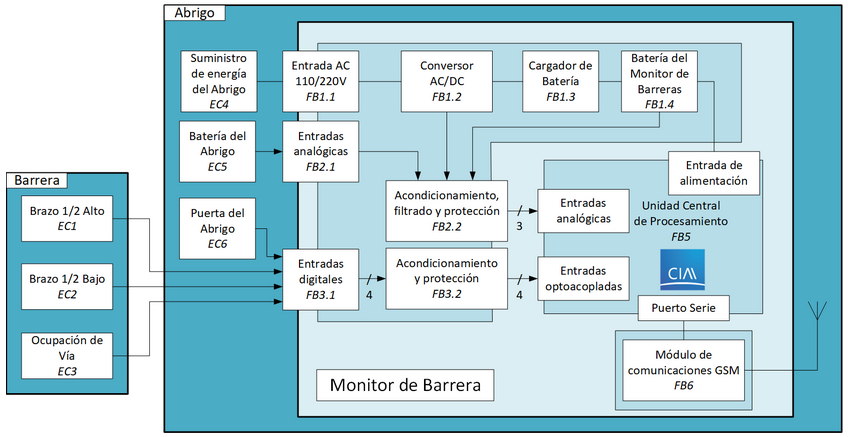
\includegraphics[width=.85\textwidth]{./Figuras/diagBloques.png}
\caption{Diagrama en bloques del sistema.}
\label{fig:diagBloques}
\end{figure}

En primer lugar, se ingesta y consolidan los datos. La información necesaria para alimentar el modelo será recopilada y unificada. El sistema se alimenta de múltiples fuentes para comprender las preferencias de cada cliente. Por un lado, analiza el historial de compras pasado, identificando qué productos han sido más relevantes para cada tipo de negocio. Por otro, incorpora señales de interacciones digitales, como búsquedas frecuentes, productos visualizados o artículos añadidos al carrito sin compra finalizada. Estos registros se complementan con características de cada punto de venta, como su ubicación geográfica, tamaño del establecimiento y perfil de clientes finales que atienden. Y, a su vez, atributos contextuales del producto, incluyendo su categoría, marca y posición dentro del portafolio. Esta etapa busca construir una base enriquecida que capture la interacción entre clientes y productos desde múltiples dimensiones.

Luego, el proceso avanza hacia la construcción de variables predictivas. En esta etapa, los datos crudos se transforman en un conjunto de features numéricos que describen la relación entre cada cliente y cada producto. Estas variables resumen comportamientos como la frecuencia y recencia de interacción, la diversidad de categorías exploradas o la intensidad de actividad en ventanas temporales relevantes. También se incorporan representaciones contextuales, como la popularidad del producto en segmentos similares o el grado de exposición previa del cliente a ese ítem. Este conjunto de features constituye la entrada del modelo de afinidad.

El tercer componente funcional corresponde al modelo de cálculo del score, que toma las variables generadas y estima un valor continuo de afinidad para cada par cliente-producto. Este score representa una medida relativa de interés y es utilizado para ordenar los productos de acuerdo a su relevancia estimada para cada punto de venta. El modelo se actualiza de forma periódica y está diseñado para adaptarse a la dinámica del negocio, incorporando señales recientes sin perder la estabilidad en el tiempo. Se utilizara el modelo desarrollado que mejores resultados obtenga.

Una vez generado el score, se realiza una etapa de evaluación y validación, donde se mide el desempeño del modelo utilizando métricas específicas del ámbito de los sistemas de recomendación. Entre las más relevantes se incluyen el recall@K, la cobertura del portafolio sugerido, la diversidad de los productos recomendados y el MAP@K. Estas métricas permiten monitorear la calidad de las recomendaciones generadas, tanto de forma global como por segmento de cliente, e identificar oportunidades de mejora en la estrategia de personalización.

Finalmente, los scores generados se integran en el flujo operativo del negocio, que organiza los resultados en rankings personalizados para cada cliente. Estos rankings pueden ser consumidos directamente por la aplicación de ventas utilizada por los puntos de venta, o bien por el equipo comercial como insumo para la planificación de sus interacciones. De este modo, el sistema aporta valor tangible al proceso comercial, permitiendo sugerencias más relevantes, focalizadas y consistentes con el comportamiento real de cada cliente.

\section{2. Identificación y análisis de los interesados}
\label{sec:interesados}

El proyecto involucra a distintos actores relevantes en su desarrollo, validación y futura aplicación.  El cliente, quien se desempeña como Director del equipo de Data en la \empclientename, es el principal impulsor de la iniciativa y sponsor del proyecto. En particular, se destaca la participación del equipo de Portfolio Strategy como usuario final del sistema, representado por su Product Owner (PO), quien actúa como principal referente funcional articulando entre los requerimientos del negocio y las decisiones técnicas. La responsable directa del desarrollo es la autora de este trabajo, quien llevará adelante el diseño, desarrollo y la implementación de la solución. La siguiente tabla resume estos roles y sus respectivas organizaciones.

\begin{table}[ht]
%\caption{Identificación de los interesados}
%\label{tab:interesados}
\begin{tabularx}{\linewidth}{@{}|l|X|X|l|@{}}
\hline
\rowcolor[HTML]{C0C0C0} 
Rol           & Nombre y Apellido & Organización 	& Puesto 	\\ \hline
% Auspiciante   &                   &              	&        	\\ \hline
Cliente       & \clientename      &\empclientename	& Gerente del Proyecto       	\\ \hline
% Impulsor      &                   &              	&        	\\ \hline
Responsable   & \authorname       & FIUBA        	& Alumno 	\\ \hline
%Colaboradores &                   &              	&        	\\ \hline
Orientador    & \supname	      & \pertesupname 	& Director del Trabajo Final \\ \hline
% Equipo        & miembro1 \newline 
%				miembro2          &              	&        	\\ \hline
% Opositores    &                   &              	&        	\\ \hline
Usuario final &  Lic. Micaela Bassan    & \empclientename	&  Product Owner \\ \hline
\end{tabularx}
\end{table}

\section{3. Propósito del proyecto}
\label{sec:proposito}

La necesidad de este proyecto surge de una limitación en la forma en que actualmente se definen las recomendaciones comerciales y la estrategia comercial. Hoy se priorizan principalmente productos ya comprados, lo que restringe el descubrimiento de nuevas oportunidades y deja sin cobertura buena parte del portafolio. Entendiendo el comportamiento cambiante de los puntos de venta y la alta rotación de catálogo, se vuelve clave contar con una herramienta que anticipe el interés de cada cliente más allá de su historial.  
En ese marco, el objetivo del proyecto es desarrollar un sistema que permita estimar la relevancia potencial de cada producto para cada punto de venta, generando rankings personalizados que orienten la planificación comercial. La implementación de esta solución permitirá mejorar la precisión de las sugerencias, ampliar la rotación de productos estratégicos y avanzar hacia una gestión más predictiva, escalable y alineada con los objetivos comerciales de la empresa.

\section{4. Alcance del proyecto}
\label{sec:alcance}

El universo sobre el cual se desarrollará esta iniciativa corresponde al conjunto de clientes y productos gestionado por el equipo de Portfolio Strategy en Argentina. Este se limita a clientes activos pertenecientes a los canales de Kioscos, Tradicionales y Autoservicios, bajo el régimen \textit{Off Premise}\footnote{Off Premise refiere a puntos de venta donde el producto es adquirido para consumo fuera del establecimiento.}. La cartera de productos considerada se enfoca exclusivamente en bebidas. Quedan excluidos del alcance los clientes de los canales \textit{On Premise}, Supermercados y Mayoristas, dado que presentan dinámicas comerciales significativamente diferentes y representan una fracción menor del total. Tampoco se contempla el negocio de marketplace, debido a sus particularidades operativas y a su peso relativamente reducido dentro del universo analizado.

El desarrollo del proyecto se organiza en una serie de etapas que abarcan desde la exploración inicial del estado del arte hasta la implementación del modelo y su evaluación en entorno real. Estas etapas permiten avanzar de forma iterativa y asegurar la calidad del entregable final, tanto desde el punto de vista técnico como funcional. A continuación, se detallan las principales actividades previstas:

\begin{itemize}
\item Relevamiento de modelos \textit{benchmark} y revisión del estado del arte.
\item Definición de métricas de éxito del proyecto.
\item Desarrollo de un modelo \textit{baseline} como punto de comparación inicial.
\item Formulación de hipótesis orientadoras del enfoque propuesto.
\item Desarrollo del proceso de \textit{feature engineering}.
\item Entrenamiento y validación de modelos.
\item Evaluación de resultados con métricas de recomendación.
\item Construcción del pipeline de implementación.
\item Ejecución de pruebas tipo A/B.
\item Reporte y presentación de resultados.
\item Registro y disponibilización del modelo final en MLflow.
\end{itemize}

Si bien este desarrollo se enmarca en un universo específico de clientes y productos, el enfoque está diseñado de manera modular, con el objetivo de facilitar su adaptación a otros segmentos del negocio en caso de resultar exitoso.

\section{5. Supuestos del proyecto}
\label{sec:supuestos}

Para el desarrollo del presente proyecto se supone que: 
\begin{itemize}
	\item Se cuenta con acceso a las fuentes de información necesarias para el desarrollo de la solución. 
	\item Se dispone con los accesos a recursos cloud y software necesarios para el desarrollo de la solución. 
	\item El tiempo asignado para completar el proyecto sera suficiente.
        \item Los colaboradores e interesados clave disponen del tiempo para reuniones de validación y toma de decisiones.
\end{itemize}

\section{6. Product Backlog}
\label{sec:backlog}

\begin{itemize}
  \item \textbf{\'{E}pica 1: \textit{Discovery} y entendimiento del problema}
    \begin{itemize}
      \item Definición de expectativas del cliente  
      \item Lectura y análisis del Estado del Arte
      \item Definición de métricas y KPIs a seguir
    \end{itemize}
  \item \textbf{\'{E}pica 2: Desarrollo de ingeniería de atributos}
    \begin{itemize}
      \item ETL
      \item EDA
      \item FE 
    \end{itemize}
  \item \textbf{\'{E}pica 3: Modelado y Evaluación}
    \begin{itemize}
      \item Desarrollo de modelo \textit{baseline}
      \item Desarrollo de modelo \textit{benchmark}
      \item Evaluación de resultados
      \item Disponibilización en MLFlow
    \end{itemize}
  \item \textbf{\'{E}pica 4: Implementación}
    \begin{itemize}
      \item Preparación de \textit{pipeline} de implementación
      \item A/B Testing
      \item Seguimiento de salubridad
      \item Presentación de resultados.
    \end{itemize}
\end{itemize}

\begin{consigna}{red} % ELIMINAR \begin{consigna}{red} y \end{consigna}{red} en las secciones que vayan completando para cada entrega parcial.

El Product Backlog debe organizarse en cuatro \textbf{\textit{\'{e}picas}} fundamentales del proyecto. Cada \'{e}pica debe contener al menos dos historias de usuario que describan funcionalidades clave.

El Product Backlog debe permitir interpretar cómo será el proyecto y su funcionalidad. Se deben indicar claramente las prioridades entre las historias de usuario y si hay alguna opcional.

Las historias de usuario deben ser breves, claras y medibles, expresando el rol, la necesidad y el propósito de cada funcionalidad. También deben tener una prioridad definida para facilitar la planificación de los sprints.

Cada historia de usuario debe incluir una ponderación en \textit{Story Points}, un número entero que representa el tama\~no relativo de la historia. El criterio para calcular los Story Points debe indicarse explícitamente.

Las historias deben seguir el formato: ``\textit{Como [rol], quiero [tal cosa] para [tal otra cosa]}''.

Las \'{e}picas deben estructurarse de la siguiente forma:

\begin{itemize}
  \item \textbf{\'{E}pica 1: \textit{Discovery} y entendimiento del problema}
    \begin{itemize}
      \item Definición de expectativas del cliente  
      \item Lectura y análisis del Estado del Arte
      \item Definición de métricas y KPIs a seguir
    \end{itemize}
  \item \textbf{\'{E}pica 2: Desarrollo de ingeniería de atributos}
    \begin{itemize}
      \item ETL
      \item EDA
      \item FE 
    \end{itemize}
  \item \textbf{\'{E}pica 3: Modelado y Evaluación}
    \begin{itemize}
      \item Desarrollo de modelo \textit{baseline}
      \item Desarrollo de modelo \textit{benchmark}
      \item Evaluación de resultados
      \item Disponibilización en MLFlow
    \end{itemize}
  \item \textbf{\'{E}pica 4: Implementación}
    \begin{itemize}
      \item Preparación de \textit{pipeline} de implementación
      \item A/B Testing
      \item Seguimiento de salubridad
      \item Presentación de resultados.
    \end{itemize}
\end{itemize}

\textbf{Reglas para definir historias de usuario:}
\begin{itemize}
  \item Ser concisas y claras.
  \item Expresarlas en términos cuantificables y medibles.
  \item No dejar margen para interpretaciones ambiguas.
  \item Indicar claramente su prioridad y si son opcionales.
  \item Considerar regulaciones y normas vigentes.
\end{itemize}

\end{consigna} % ELIMINAR \begin{consigna}{red} y \end{consigna}{red} en las secciones que vayan completando para cada entrega parcial.


\section{7. Criterios de aceptación de historias de usuario}
\label{sec:criteriosAceptacion}

\begin{consigna}{red} % ELIMINAR \begin{consigna}{red} y \end{consigna}{red} en las secciones que vayan completando para cada entrega parcial.

Los criterios de aceptación deben establecerse para cada historia de usuario, asegurando que se cumplan las condiciones necesarias para que la funcionalidad sea validada correctamente.

Cada historia debe tener criterios medibles, específicos y verificables. Deben permitir validar que se cumple con las necesidades del usuario.

Se estructuran de forma análoga a las \'{e}picas del backlog:

\begin{itemize}
  \item \textbf{\'{E}pica 1}
    \begin{itemize}
      \item Criterios de aceptación HU1
      \item Criterios de aceptación HU2
    \end{itemize}
  \item \textbf{\'{E}pica 2}
    \begin{itemize}
      \item Criterios de aceptación HU3
      \item Criterios de aceptación HU4
    \end{itemize}
  \item \textbf{\'{E}pica 3}
    \begin{itemize}
      \item Criterios de aceptación HU5
      \item Criterios de aceptación HU6
    \end{itemize}
  \item \textbf{\'{E}pica 4}
    \begin{itemize}
      \item Criterios de aceptación HU7
      \item Criterios de aceptación HU8
    \end{itemize}
\end{itemize}

\textbf{Reglas para definir criterios de aceptación:}
\begin{itemize}
  \item Medibles y verificables.
  \item Especificar cuándo una historia se considera completada.
  \item Incluir condiciones específicas.
  \item No ambiguos.
  \item Probables de testear funcional o técnicamente.
  \item Mínimo 3 criterios por HU.
\end{itemize}

\end{consigna} % ELIMINAR \begin{consigna}{red} y \end{consigna}{red} en las secciones que vayan completando para cada entrega parcial.


\section{8. Fases de CRISP-DM}

\begin{consigna}{red} % ELIMINAR \begin{consigna}{red} y \end{consigna}{red} en las secciones que vayan completando para cada entrega parcial.

\begin{enumerate}
  \item \textbf{Comprensión del negocio:} objetivo, valor agregado de IA, métricas de éxito.
  \item \textbf{Comprensión de los datos:} tipo, origen, cantidad, calidad.
  \item \textbf{Preparación de los datos:} características clave, transformaciones necesarias.
  \item \textbf{Modelado:} tipo de problema, algoritmos posibles.
  \item \textbf{Evaluación del modelo:} métricas de rendimiento.
  \item \textbf{Despliegue del modelo (opcional):} tipo de despliegue y herramientas.
\end{enumerate}

\end{consigna} % ELIMINAR \begin{consigna}{red} y \end{consigna}{red} en las secciones que vayan completando para cada entrega parcial.


\section{9. Desglose del trabajo en tareas}
\label{sec:wbs}

\begin{consigna}{red} % ELIMINAR \begin{consigna}{red} y \end{consigna}{red} en las secciones que vayan completando para cada entrega parcial.

A partir de cada HU, descomponer en tareas concretas, técnicas y medibles:

\begin{itemize}
  \item Duración estimada: entre 2 y 8 h. Evitar tareas genéricas.
  \item Si una tarea excede 8 h, dividirla.
  \item Indicar prioridad relativa (Alta, Media, Baja).
\end{itemize}

\begin{table}[htpb]
\centering
\begin{tabularx}{\linewidth}{@{}|X|X|c|c|@{}}
\hline
\rowcolor[HTML]{C0C0C0}
Historia de usuario & Tarea técnica & Estimación & Prioridad \\ \hline
HU1 & Tarea 1 HU1 & 6 h & Alta \\ \hline
HU1 & Tarea 2 HU1 & 8 h & Alta \\ \hline
HU2 & Tarea 1 HU2 & 5 h & Media \\ \hline
HU2 & Tarea 2 HU2 & 6 h & Alta \\ \hline
... & ... & ... & ... \\ \hline
\end{tabularx}
\end{table}

\textbf{Criterios para estimar tiempos:}
\begin{itemize}
  \item Considerar dificultad, complejidad técnica y grado de incertidumbre de cada tarea.
  \item Evitar subestimar el esfuerzo requerido. Si una tarea supera las 8 h, dividirla en subtareas.
  \item Basar la estimación en la experiencia propia o en referencias de tareas similares.
\end{itemize}

\textbf{Sobre la prioridad:}
\begin{itemize}
  \item Asignar una prioridad relativa (Alta, Media o Baja) según la relevancia funcional de la tarea y su impacto en los entregables.
  \item Priorizar tareas que estén vinculadas a criterios de aceptación de las HU o que sean necesarias para desbloquear otras.
  \item Incluir tareas opcionales solo si están bien justificadas.
\end{itemize}

\textbf{Recomendaciones generales:}
\begin{itemize}
  \item Incluir al menos dos tareas por historia de usuario.
  \item El total estimado debe ser coherente con la planificación global de unas 600 horas (la cantidad de horas sugeridas para un trabajo de posgrado).
  \item Este desglose se utilizará en las secciones siguientes para armar el diagrama de Gantt (sección 10) y la planificación de sprints (sección 11).
  \item Recordar que la calidad del desglose impacta directamente en la calidad de la planificación del proyecto.
\end{itemize}

\end{consigna} % ELIMINAR \begin{consigna}{red} y \end{consigna}{red} en las secciones que vayan completando para cada entrega parcial.


\section{10. Diagrama de Gantt}
\label{sec:gantt}

\begin{consigna}{red} % ELIMINAR \begin{consigna}{red} y \end{consigna}{red} en las secciones que vayan completando para cada entrega parcial.

El diagrama de Gantt debe representar de forma visual y cronológica todas las tareas del proyecto, abarcando aproximadamente 600 horas totales, de las cuales entre 480 y 500 deben destinarse a tareas técnicas (desarrollo, pruebas, implementación) y entre 100 y 120 a tareas no técnicas (planificación, documentación, escritura de memoria y preparación de la defensa).

\textbf{Consignas y recomendaciones:}
\begin{itemize}
  \item Incluir tanto tareas técnicas derivadas de las HU como tareas no técnicas generales del proyecto.
  \item El eje vertical debe listar las tareas y el eje horizontal representar el tiempo en semanas o fechas.
  \item Utilizar colores diferenciados para distinguir tareas técnicas y no técnicas.
  \item Las tareas deben estar ordenadas cronológicamente y reflejar todo el ciclo del proyecto.
  \item Iniciar con la planificación del proyecto (coincidente con el inicio de Gestión de Proyectos) y finalizar con la defensa, próxima a la fecha de cierre del trabajo.
  \item Configurar el software para mostrar los códigos del desglose de tareas y los nombres junto a cada barra.
  \item Asegurarse de que la fecha final coincida con la del Acta Constitutiva.
  \item Evitar tareas genéricas o ambiguas y asegurar una secuencia lógica y realista.
  \item Las fechas pueden ser aproximadas; ajustar el ancho del diagrama según el texto y el parámetro \texttt{x unit}. Para mejorar la apariencia del diagrama, es necesario ajustar este valor y, quizás, acortar los nombres de las tareas.
\end{itemize}

\textbf{Herramientas sugeridas:}
\begin{itemize}
  \item Planner, GanttProject, Trello + plugins\\
  \url{https://blog.trello.com/es/diagrama-de-gantt-de-un-proyecto}
  \item Creately (colaborativa online)\\
  \url{https://creately.com/diagram/example/ieb3p3ml/LaTeX}
  \item LaTeX con \texttt{pgfgantt}:\\
  \url{http://ctan.dcc.uchile.cl/graphics/pgf/contrib/pgfgantt/pgfgantt.pdf}
\end{itemize}

Incluir una imagen legible del diagrama de Gantt. Si es muy ancho, presentar primero la tabla y luego el gráfico de barras.

\end{consigna} % ELIMINAR \begin{consigna}{red} y \end{consigna}{red} en las secciones que vayan completando para cada entrega parcial.


\section{11. Planificación de Sprints}

\begin{consigna}{red} % ELIMINAR \begin{consigna}{red} y \end{consigna}{red} en las secciones que vayan completando para cada entrega parcial.

Organizar las tareas técnicas del proyecto en sprints de trabajo que permitan distribuir de forma equilibrada la carga horaria total, estimada en 600 horas.

\textbf{Consigna:}
\begin{itemize}
  \item Completar una tabla que relacione sprints con HU y tareas técnicas correspondientes.
  \item Incluir estimación en horas para cada tarea.
  \item Indicar responsable y porcentaje de avance estimado o completado.
  \item Contemplar también tareas de planificación, documentación, redacción de memoria y preparación de defensa.
\end{itemize}

\textbf{Conceptos clave:}
\begin{itemize}
  \item Una \'{e}pica es una unidad funcional amplia; una historia de usuario es una funcionalidad concreta; un sprint es una unidad de tiempo donde se ejecutan tareas.
  \item Las tareas son el nivel más desagregado: permiten estimar tiempos, asignar responsables y monitorear progreso.
\end{itemize}

\textbf{Duración sugerida:}
\begin{itemize}
  \item Para un proyecto de 600 h, se recomienda planificar entre 10 y 12 sprints de aproximadamente 2 semanas cada uno.
  \item Asignar entre 45 y 50 horas efectivas por sprint a tareas técnicas.
  \item Reservar 100 a 120 h para actividades no técnicas (planificación, escritura, reuniones, defensa).
\end{itemize}

\textbf{Importante:}
\begin{itemize}
  \item En proyectos individuales, el responsable suele ser el propio autor.
  \item Aun así, desagregar tareas facilita el seguimiento y mejora continua.
\end{itemize}

\textbf{Conversión opcional de Story Points a horas:}
\begin{itemize}
  \item 1 SP \(\approx\) 2 h como referencia flexible.
  \item Tener en cuenta aproximaciones tipo Fibonacci.
\end{itemize}

\begin{table}[htpb]
\centering
\caption{Formato sugerido}
\begin{tabularx}{\linewidth}{@{}|l|l|X|c|l|c|@{}}
\hline
\rowcolor[HTML]{C0C0C0}
Sprint & HU o fase & Tarea & Horas / SP & Responsable & \% Completado \\ \hline
Sprint 0 & Planificación & Definir alcance y cronograma & 10 h & Alumno & 100\% \\ \hline
Sprint 0 & Planificación & Reunión con tutor/cliente & 5 h & Alumno & 50\% \\ \hline
Sprint 0 & Planificación & Ajuste de entregables & 6 h & Alumno & 25\% \\ \hline
Sprint 1 & HU1 & Tarea 1 HU1 & 6 h / 3 SP & Alumno & 0\% \\ \hline
Sprint 1 & HU1 & Tarea 2 HU1 & 10 h / 5 SP & Alumno & 0\% \\ \hline
Sprint 2 & HU2 & Tarea 1 HU2 & 7 h / 5 SP & Alumno & 0\% \\ \hline
... & ... & ... & ... & ... & ... \\ \hline
Sprint 5 & Escritura & Redacción memoria & 50 h / 34 SP & Alumno & 0\% \\ \hline
Sprint 6 & Defensa & Preparación exposición & 20 h / 13 SP & Alumno & 0\% \\ \hline
\end{tabularx}
\end{table}

\textbf{Recomendaciones:}
\begin{itemize}
  \item Verificar que la carga horaria por sprint sea equilibrada.
  \item Usar sprints de 1 a 3 semanas, acordes al cronograma general.
  \item Actualizar el \% completado durante el seguimiento del proyecto.
  \item Considerar un sprint final exclusivo para pruebas, revisión y ajustes antes de la defensa.
\end{itemize}

\end{consigna} % ELIMINAR \begin{consigna}{red} y \end{consigna}{red} en las secciones que vayan completando para cada entrega parcial.


\section{12. Normativa y cumplimiento de datos (gobernanza)}

\begin{consigna}{red} % ELIMINAR \begin{consigna}{red} y \end{consigna}{red} en las secciones que vayan completando para cada entrega parcial.

En esta sección se debe analizar si los datos utilizados en el proyecto están sujetos a normativas de protección de datos y privacidad, y en qué condiciones se pueden emplear.

\textbf{Aspectos a considerar:}
\begin{itemize}
  \item Evaluar si los datos están regulados por normativas como GDPR, Ley 25.326 de Protección de Datos Personales en Argentina, HIPAA u otras según jurisdicción y temática.
  \item Determinar si el uso de los datos requiere consentimiento explícito de los usuarios involucrados.
  \item Indicar si existen restricciones legales, técnicas o contractuales sobre el uso, compartición o publicación de los datos.
  \item Aclarar si los datos provienen de fuentes licenciadas, de acceso público o bajo algún tipo de autorización especial.
  \item Analizar la viabilidad del proyecto desde el punto de vista legal y ético, considerando la gobernanza de los datos.
\end{itemize}

Este análisis es clave para garantizar el cumplimiento normativo y evitar conflictos legales durante el desarrollo y publicación del proyecto.

\end{consigna} % ELIMINAR \begin{consigna}{red} y \end{consigna}{red} en las secciones que vayan completando para cada entrega parcial.

\section{13. Gestión de riesgos}
\label{sec:riesgos}

\begin{consigna}{red} % ELIMINAR \begin{consigna}{red} y \end{consigna}{red} en las secciones que vayan completando para cada entrega parcial.
a) Identificación de los riesgos (al menos cinco) y estimación de sus consecuencias:
 
Riesgo 1: detallar el riesgo (riesgo es algo que si ocurre altera los planes previstos de forma negativa)
\begin{itemize}
	\item Severidad (S): mientras más severo, más alto es el número (usar números del 1 al 10).\\
	Justificar el motivo por el cual se asigna determinado número de severidad (S).
	\item Probabilidad de ocurrencia (O): mientras más probable, más alto es el número (usar del 1 al 10).\\
	Justificar el motivo por el cual se asigna determinado número de (O). 
\end{itemize}   

Riesgo 2:
\begin{itemize}
	\item Severidad (S): X.\\
	Justificación...
	\item Ocurrencia (O): Y.\\
	Justificación...
\end{itemize}

Riesgo 3:
\begin{itemize}
	\item Severidad (S):  X.\\
	Justificación...
	\item Ocurrencia (O): Y.\\
	Justificación...
\end{itemize}


b) Tabla de gestión de riesgos:      (El RPN se calcula como RPN=SxO)

\begin{table}[htpb]
\centering
\begin{tabularx}{\linewidth}{@{}|X|c|c|c|c|c|c|@{}}
\hline
\rowcolor[HTML]{C0C0C0} 
Riesgo & S & O & RPN & S* & O* & RPN* \\ \hline
       &   &   &     &    &    &      \\ \hline
       &   &   &     &    &    &      \\ \hline
       &   &   &     &    &    &      \\ \hline
       &   &   &     &    &    &      \\ \hline
       &   &   &     &    &    &      \\ \hline
\end{tabularx}%
\end{table}

Criterio adoptado: 

Se tomarán medidas de mitigación en los riesgos cuyos números de RPN sean mayores a...

Nota: los valores marcados con (*) en la tabla corresponden luego de haber aplicado la mitigación.

c) Plan de mitigación de los riesgos que originalmente excedían el RPN máximo establecido:
 
Riesgo 1: plan de mitigación (si por el RPN fuera necesario elaborar un plan de mitigación).
  Nueva asignación de S y O, con su respectiva justificación:
  \begin{itemize}
	\item Severidad (S*): mientras más severo, más alto es el número (usar números del 1 al 10).
          Justificar el motivo por el cual se asigna determinado número de severidad (S).
	\item Probabilidad de ocurrencia (O*): mientras más probable, más alto es el número (usar del 1 al 10).
          Justificar el motivo por el cual se asigna determinado número de (O).
	\end{itemize}

Riesgo 2: plan de mitigación (si por el RPN fuera necesario elaborar un plan de mitigación).
 
Riesgo 3: plan de mitigación (si por el RPN fuera necesario elaborar un plan de mitigación).

\end{consigna} % ELIMINAR \begin{consigna}{red} y \end{consigna}{red} en las secciones que vayan completando para cada entrega parcial.


\section{14. Sprint Review}
\label{sec:sprint_review}

\begin{consigna}{red} % ELIMINAR \begin{consigna}{red} y \end{consigna}{red} en las secciones que vayan completando para cada entrega parcial.

La revisión de sprint (\emph{Sprint Review}) es una práctica fundamental en metodologías ágiles. Consiste en revisar y evaluar lo que se ha completado al finalizar un sprint. En esta instancia, se presentan los avances y se verifica si las funcionalidades cumplen con los criterios de aceptación establecidos. También se identifican entregables parciales y se consideran ajustes si es necesario.

Aunque el proyecto aún se encuentre en etapa de planificación, esta sección permite proyectar cómo se evaluarán las funcionalidades más importantes del backlog. Esta mirada anticipada favorece la planificación enfocada en valor y permite reflexionar sobre posibles obstáculos.

\textbf{Objetivo:} anticipar cómo se evaluará el avance del proyecto a medida que se desarrollen las funcionalidades, utilizando como base al menos cuatro historias de usuario del \emph{Product Backlog}.


Seleccionar al menos 4 HU del Product Backlog. Para cada una, completar la siguiente tabla de revisión proyectada:

\textbf{Formato sugerido:}
\begin{table}[htpb]
\renewcommand{\arraystretch}{1.5}
\begin{tabular}{|>{\raggedright\arraybackslash}m{2.5cm}|
                >{\raggedright\arraybackslash}m{2.3cm}|
                >{\raggedright\arraybackslash}m{3cm}|
                >{\raggedright\arraybackslash}m{3cm}|
                >{\raggedright\arraybackslash}m{3cm}|}
\hline
\rowcolor[HTML]{CCCCCC}
\textbf{HU seleccionada} & \textbf{Tareas asociadas} & \textbf{Entregable esperado} & \textbf{¿Cómo sabrás que está cumplida?} & \textbf{Observaciones o riesgos} \\
\hline
                         & Tarea 1 &                             &                                           &                                     \\ \cline{2-2}
\multirow{-2}{=}{HU1}    & Tarea 2 & \multirow{-2}{=}{Módulo funcional} & \multirow{-2}{=}{Cumple criterios de aceptación definidos} & \multirow{-2}{=}{Falta validar con el tutor} \\
\hline
                         & Tarea 1 &                             &                                           &                                     \\ \cline{2-2}
\multirow{-2}{=}{HU3}    & Tarea 2 & \multirow{-2}{=}{Reporte generado} & \multirow{-2}{=}{Exportación disponible y clara} & \multirow{-2}{=}{Requiere datos reales} \\
\hline
                         & Tarea 1 &                             &                                           &                                     \\ \cline{2-2}
\multirow{-2}{=}{HU5}    & Tarea 2 & \multirow{-2}{=}{Panel de gestión} & \multirow{-2}{=}{Roles diferenciados operativos} & \multirow{-2}{=}{Riesgo en integración} \\
\hline
                         & Tarea 1 &                             &                                           &                                     \\ \cline{2-2}
\multirow{-2}{=}{HU7}    & Tarea 2 & \multirow{-2}{=}{Informe trimestral} & \multirow{-2}{=}{PDF con gráficos y evolución} & \multirow{-2}{=}{Puede faltar tiempo para ajustes} \\
\hline
\end{tabular}
\end{table}

\end{consigna} % ELIMINAR \begin{consigna}{red} y \end{consigna}{red} en las secciones que vayan completando para cada entrega parcial.


\section{15. Sprint Retrospective}    
\label{sec:sprint_retro}

\begin{consigna}{red} % ELIMINAR \begin{consigna}{red} y \end{consigna}{red} en las secciones que vayan completando para cada entrega parcial.

La retrospectiva de sprint es una práctica orientada a la mejora continua. Al finalizar un sprint, el equipo (o el alumno, si trabaja de forma individual) reflexiona sobre lo que funcionó bien, lo que puede mejorarse y qué acciones concretas pueden implementarse para trabajar mejor en el futuro.

Durante la cursada se propuso el uso de la \textbf{Estrella de la Retrospectiva}, que organiza la reflexión en torno a cinco ejes:

\begin{itemize}
\item  ¿Qué hacer más?
\item  ¿Qué hacer menos?
\item  ¿Qué mantener?
\item  ¿Qué empezar a hacer?
\item  ¿Qué dejar de hacer?
\end{itemize}

Aun en una etapa temprana, esta herramienta permite que el alumno planifique su forma de trabajar, identifique anticipadamente posibles dificultades y diseñe estrategias de organización personal.

\textbf{Objetivo:} reflexionar sobre las condiciones iniciales del proyecto, identificando fortalezas, posibles dificultades y estrategias de mejora, incluso antes del inicio del desarrollo.


Completar la siguiente tabla tomando como referencia los cinco ejes de la Estrella de la Retrospectiva (\emph{Starfish} o estrella de mar). Esta instancia te ayudará a definir buenas prácticas desde el inicio y prepararte para enfrentar el trabajo de forma organizada y flexible. Se deberá completar la tabla al menos para 3 sprints técnicos y 1 no técnico.

\textbf{Formato sugerido:}

\begin{table}[htpb]
\renewcommand{\arraystretch}{1.4}
\begin{tabular}{|>{\raggedright\arraybackslash}p{1.8cm}|
                >{\raggedright\arraybackslash}p{2.3cm}|
                >{\raggedright\arraybackslash}p{2.3cm}|
                >{\raggedright\arraybackslash}p{2.3cm}|
                >{\raggedright\arraybackslash}p{2.3cm}|
                >{\raggedright\arraybackslash}p{2.3cm}|}
\hline
\rowcolor[HTML]{CCCCCC} 
\textbf{Sprint tipo y N°} & \textbf{¿Qué hacer más?} & \textbf{¿Qué hacer menos?} & \textbf{¿Qué mantener?} & \textbf{¿Qué empezar a hacer?} & \textbf{¿Qué dejar de hacer?} \\
\hline
Sprint técnico - 1 & Validaciones continuas con el alumno & Cambios sin versión registrada & Pruebas con datos simulados & Documentar cambios propuestos & Ajustes sin análisis de impacto \\
\hline
Sprint técnico - 2 & Verificar configuraciones en múltiples escenarios & Modificar parámetros sin guardar historial & Perfiles reutilizables & Usar logs para configuración & Repetir pruebas manuales innecesarias \\
\hline
Sprint técnico - 8 & Comparar correlaciones con casos previos & Cambiar parámetros sin justificar & Revisión cruzada de métricas & Anotar configuraciones usadas & Trabajar sin respaldo de datos \\
\hline
Sprint no técnico - 12 (por ej.: ``Defensa'') & Ensayos orales con feedback & Cambiar contenidos en la memoria & Material visual claro & Dividir la presentación por bloques & Agregar gráficos difíciles de explicar \\
\hline
\end{tabular}
\end{table}

\end{consigna} % ELIMINAR \begin{consigna}{red} y \end{consigna}{red} en las secciones que vayan completando para cada entrega parcial.

\end{document}